
% This LaTeX was auto-generated from MATLAB code.
% To make changes, update the MATLAB code and republish this document.

\documentclass{article}
\usepackage{graphicx}
\usepackage{color}

\sloppy
\definecolor{lightgray}{gray}{0.5}
\setlength{\parindent}{0pt}

\begin{document}

    
    \begin{par}
Minima och maxima vid punkterna $[-5, 5]$ för funktionen
\end{par} \vspace{1em}
\begin{par}
$$ f(x) = \frac{x^2 - 2x}{x^4 + 1} $$
\end{par} \vspace{1em}
\begin{verbatim}
x = linspace(-5, 5, 1000);
x1 = -5;
x2 = 5;
y = @(x) (x.^2 - 2*x) ./ (x.^4 + 1);
x_min = fminbnd(@(x) y(x), x1, x2);
x_max = fminbnd(@(x) -y(x), x1, x2);

figure;
plot(x, y(x));
hold on;
xlabel('x');
ylabel('y');
grid on;
plot(x_min, y(x_min), 'ro', 'MarkerSize', 3, 'MarkerFaceColor', 'r');
plot(x_max, y(x_max), 'ro', 'MarkerSize', 3, 'MarkerFaceColor', 'r');
hold off;
\end{verbatim}

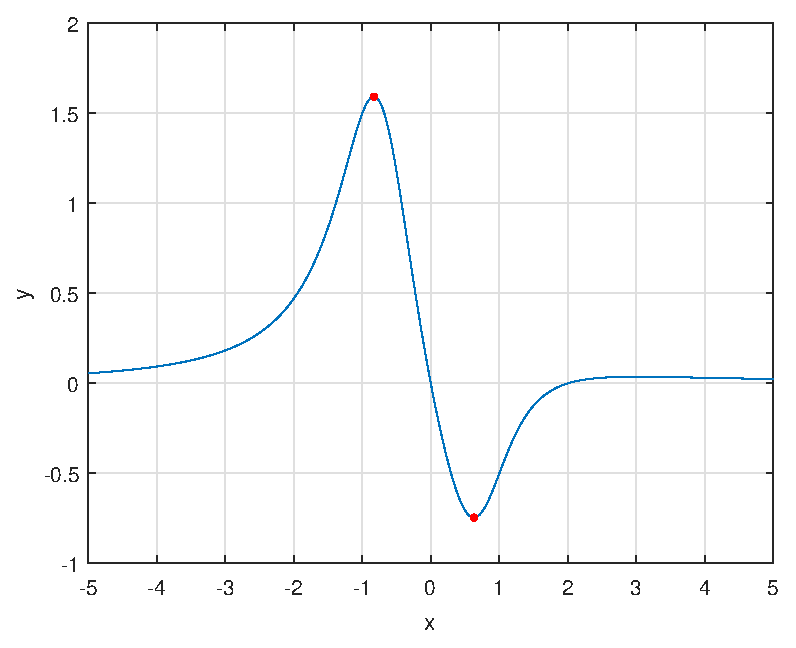
\includegraphics [width=4in]{uppg6_01.eps}
\begin{par}
Genom att använda fminbnd() så hittar vi minima genom att passera originala funktionen som argument. För att hitta maxima så passerar vi också funktionen som argument, men vi multiplicerar den med -1 för att hitta maxima, alltså omvandlar vi funktionen till $-f(x)$.
\end{par} \vspace{1em}
\begin{par}
Nu tittar vi närmare på vardera punkt
\end{par} \vspace{1em}
\begin{verbatim}
figure;
plot(x, y(x));
hold on;
xlabel('x');
ylabel('y');
grid on;
plot(x_max, y(x_max), 'ro', 'MarkerSize', 3, 'MarkerFaceColor', 'r');
axis([-0.9 -0.75, 1.5 1.65]);
hold off;
\end{verbatim}

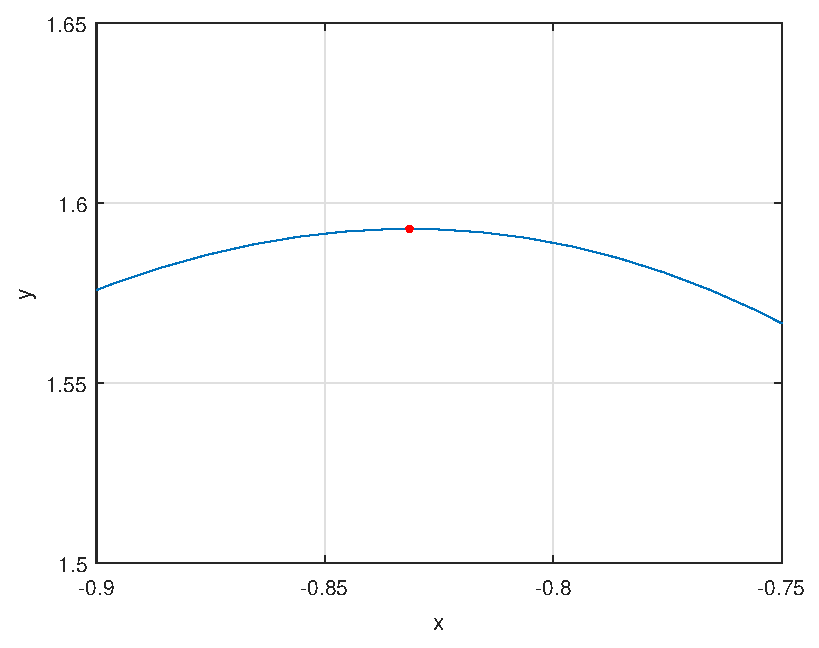
\includegraphics [width=4in]{uppg6_02.eps}
\begin{par}
$$ x_{max} \approx -0.83 $$
\end{par} \vspace{1em}
\begin{verbatim}
figure;
plot(x, y(x));
hold on;
xlabel('x');
ylabel('y');
grid on;
plot(x_min, y(x_min), 'ro', 'MarkerSize', 3, 'MarkerFaceColor', 'r');
axis([0.55 0.7, -0.8 -0.65]);
hold off;
\end{verbatim}

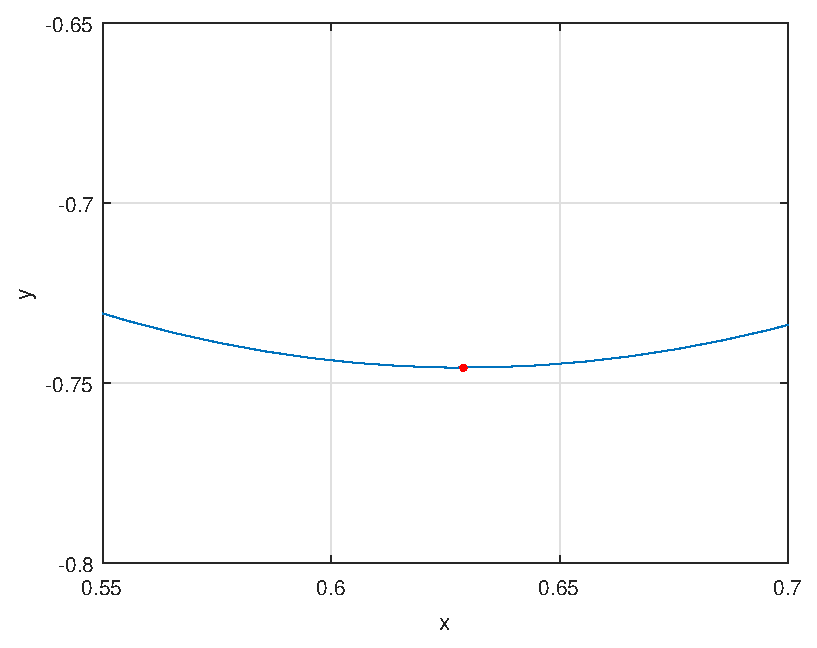
\includegraphics [width=4in]{uppg6_03.eps}
\begin{par}
$$ x_{min} \approx 0.629 $$
\end{par} \vspace{1em}
\begin{par}
Vi har alltså fått att
\end{par} \vspace{1em}
\begin{par}
$$ x_{min} \approx 0.629,~f(x_{min}) \approx -0.746 $$
\end{par} \vspace{1em}
\begin{par}
och
\end{par} \vspace{1em}
\begin{par}
$$ x_{max} \approx -0.831,~f(x_{max}) \approx 1.593. $$
\end{par} \vspace{1em}



\end{document}

